\newpage
\section{Relazioni su un insieme}
\begin{definition}[Relazioni su un insieme]
Dato un insieme $A$, una relazione su un insieme $A$ è un sottoinsieme $A \times A$, cioè un elemento di $rel(A,A)$, dove $rel(A,A)$ è l'insieme delle possibili relazioni $A \times A$. Quindi una relazione $R \subseteq A \times A$.
\end{definition}
Le relazioni su insiemi sono caratterizzate dal fatto che si sviluppano fra due insiemi uguali. Infatti non è una relazione su un insieme un $R \subseteq$ A X B.
\begin{example}
Alcuni esempi generali di relazioni su un insieme:
\begin{itemize}
    \item Succ = $\{(x,y) \in \mathbb{N} \times \mathbb{N} \mid y=x+1\}$
    \item $id_A \in rel(A,A)$ è una relazione su $A$
    \item $S$ è l'insieme degli studenti. CompagnoDiClasse $\in rel(S,S)$
    \item Somma $\in$ rel(($\mathbb{Z}, \mathbb{Z}$), $\mathbb{Z}$) Somma \textbf{NON} è una relazione su in inseme.
\end{itemize}
\end{example}

\subsection{Proprietà di relazione su un insieme}
\subsubsection{Riflessiva}
Dato un inseme $A$, una relazione $R: A \rightarrow A$ possiamo definirla come:
\begin{definition}[Riflessiva]
    R è una relazione \textbf{riflessiva} se per tutti gli $a \in A$ vale che $(a, a) \in R$
    \begin{center}
        $\forall \: a \in A . (a, a) \in R$
    \end{center}
\end{definition}
Rappresentiamo \textbf{graficamente} ora una relazione riflessiva. \\Dato un insieme $A$ di partenza dove $A = \{a, b, c, d\}$:
\begin{itemize}
    \item Il caso [\ref{fig:relazione-riflessiva}] è riflessivo perché ogni elemento è collegato a se stesso \footnote{Il collegamento di un elemento a se stesso viene anche chiamata cappio}.
    \item Il caso [\ref{fig:relazione-non-riflessiva}] \textbf{non} è riflessivo perché gli elementi $c$ e $b$ non sono collegati con loro stesso.
\end{itemize}
\begin{figure}[h!]
    \vspace{-15pt}
    \centering
    \begin{subfigure}{.3\textwidth}
        \centering
        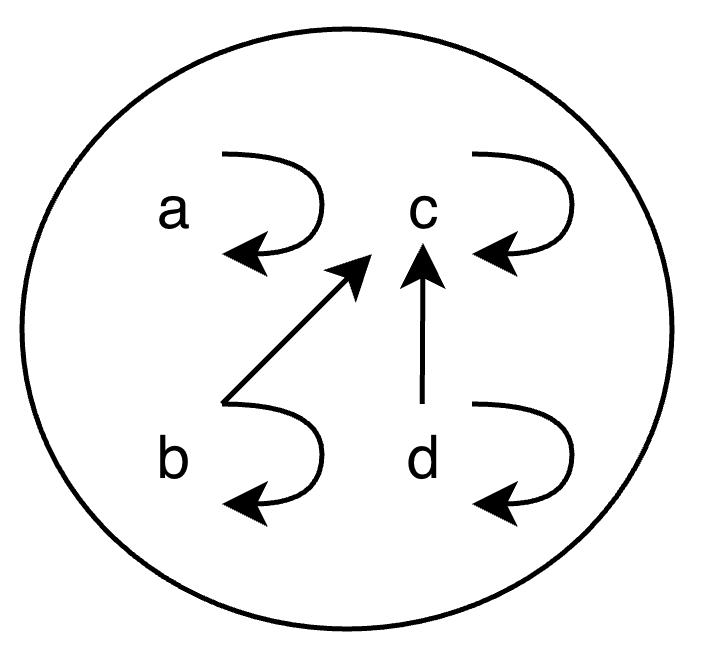
\includegraphics[width=3cm]{images/relazione-riflessiva.png}
        \caption{Relazione riflessiva}
        \label{fig:relazione-riflessiva}
    \end{subfigure}
    \hspace{1.5cm}
    \begin{subfigure}{.3\textwidth}
        \centering
        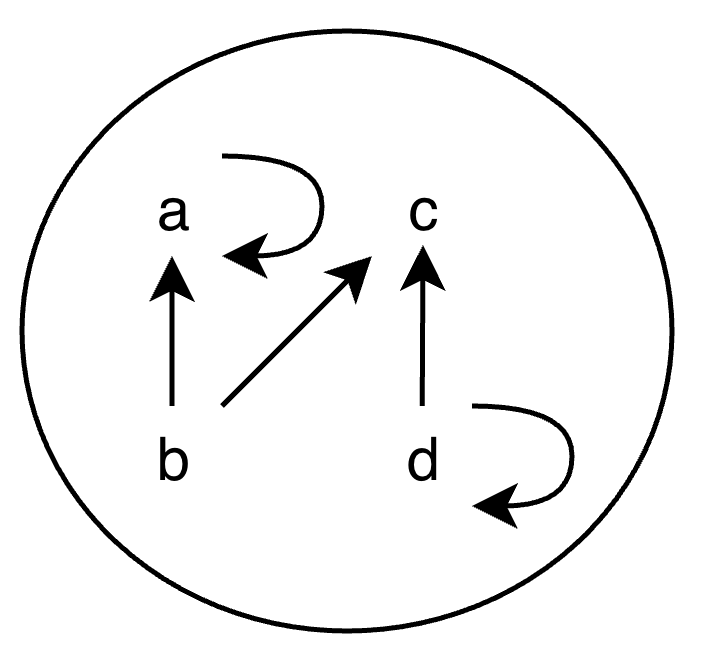
\includegraphics[width=3cm]{images/relazione-non-riflessiva.png}
        \caption{Relazione non riflessiva}
        \label{fig:relazione-non-riflessiva}
    \end{subfigure}
\end{figure}
\begin{example}
Alcuni esempi di relazioni riflessive:
    \begin{itemize}
        \item L'Identità di A $Id_A: A \leftrightarrow A$ è riflessiva.
        \item La relazione completa $A \times A:A \leftrightarrow A$ è riflessiva.
        \item La relazione vuota $\O: A \leftrightarrow A$ non è riflessiva perché non ci sono relazioni fra elementi. Se $A = \O$ allora sarebbe stata riflessiva.
        \item La relazione minore stretto $<: \mathbb{N} \leftrightarrow \mathbb{N}$ \footnote{La relazione minore è definita come: $< = \{(x,y) \in \mathbb{N}$ X $\mathbb{N}\:|\: x < y\}$} non è riflessiva perché un numero non è minore di se stesso.
        \item La relazione minore-uguale $\leq: \mathbb{N} \leftrightarrow \mathbb{N}$ \footnote{La relazione minore-uguale è definita come: $\leq = \{(x,y) \in \mathbb{N}$ X $\mathbb{N}\:|\: x \leq y\}$} è riflessiva.
        \item La relazione madre: $EU \leftrightarrow EU$ non è riflessiva.
    \end{itemize}
\end{example}

\newpage
\subsubsection{Simmetrica}
Dato un inseme A, una relazione $R: A \leftrightarrow A$ possiamo definirla come:
\begin{definition}[Simmetrica]
    R è una relazione \textbf{simmetrica} se per tutti gli $a,b \in A$ vale che se $(a, b) \in R$ allora $(b,a) \in R$.
    \begin{center}
        $\forall \: a,b \in A . (a, b) \in R \Rightarrow (b,a) \in R$
    \end{center}
\end{definition}
Rappresentiamo \textbf{graficamente} ora una relazione simmetrica. \\Dato un insieme A di partenza dove A = $\{a, b, c, d\}$:
\begin{itemize}
    \item Il caso [\ref{fig:relazione-simmetrica}] è simmetrica perché ogni elemento esiste la coppia inversa di ogni collegamento.
    \item Il caso [\ref{fig:relazione-non-simmetrica}] non è simmetrica perché gli elementi $c$ e $d$ hanno un collegamento sono in un verso.
\end{itemize}
\begin{figure}[h!]
    \vspace{-10pt}
    \centering
    \begin{subfigure}{.3\textwidth}
        \centering
        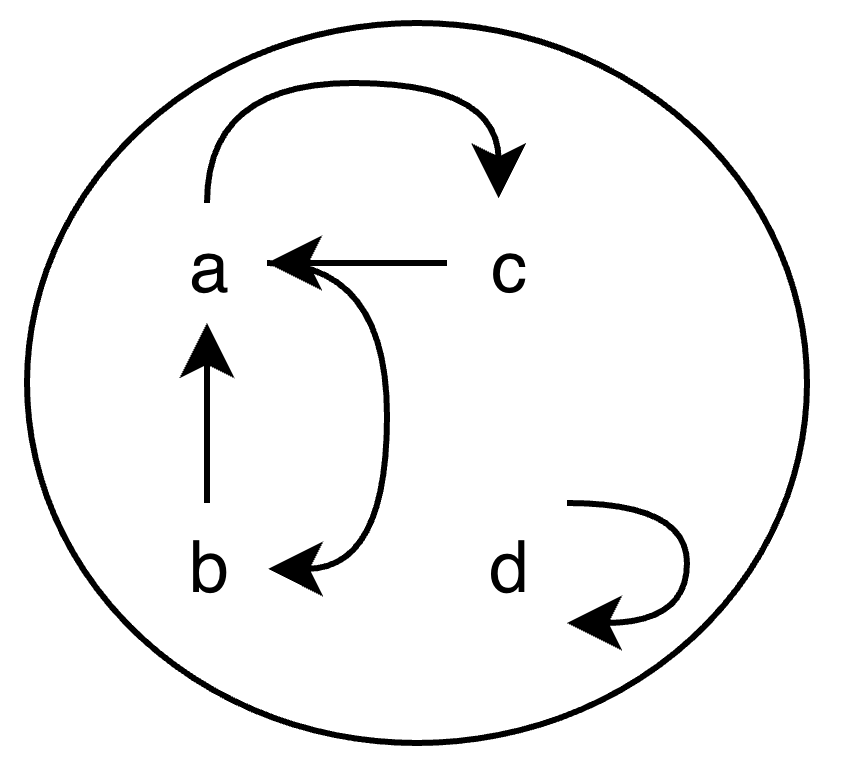
\includegraphics[width=3cm]{images/relazione-simmetrica.png}
        \caption{Relazione simmetrica}
        \label{fig:relazione-simmetrica}
    \end{subfigure}
    \hspace{1.5cm}
    \begin{subfigure}{.3\textwidth}
        \centering
        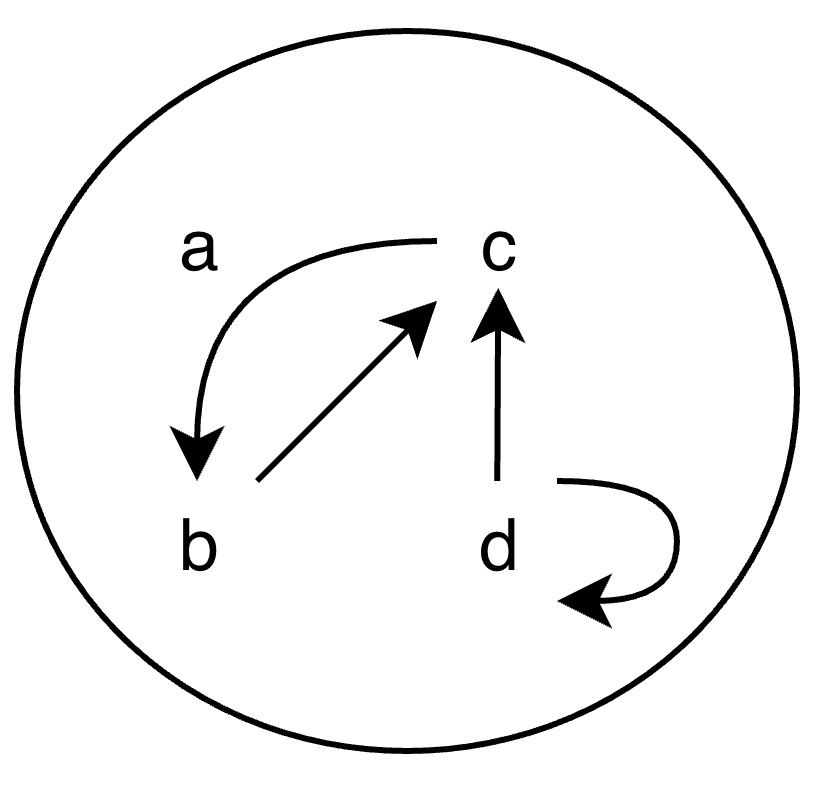
\includegraphics[width=3cm]{images/relazione-non-simmetrica.png}
        \caption{Relazione non simmetrica}
        \label{fig:relazione-non-simmetrica}
    \end{subfigure}
\end{figure}
\begin{example}
Alcuni esempi di relazioni simmetrica:
    \begin{itemize}
        \item L'Identità di $A Id_A: A \rightarrow A$ è simmetrica.
        \item La relazione completa $A \times A:A \rightarrow A$ è simmetrica.
        \item La relazione vuota $\O: A \rightarrow A$ è simmetrica.
        \item La relazione minore stretto $<: \mathbb{N} \longleftrightarrow \mathbb{N}$ non è simmetrica perché se un elemento $a$ è minore di un elemento $b$ non può essere che esista l'inverso.
        \item La relazione minore-uguale $\leq: \mathbb{N} \leftrightarrow \mathbb{N}$ non è riflessiva perché ci sono casi in cui $a$ è minore di un elemento $b$ che non permettono l'inverso.
        \item La relazioni di amicizia su facebook FbFreind:FB $\longleftrightarrow$ FB è simmetrica.
        \item La relazioni di follow su instagram IGFollow:IG $\longleftrightarrow$ IG non è simmetrica perchè se te sei follow di un utente questo utente non necessariamente lo è di te.
    \end{itemize}
\end{example}

\subsubsection{Transitiva}
Dato un inseme A, una relazione $R: A \leftrightarrow A$ possiamo definirla come:
\begin{definition}[Transitiva]
    R è una relazione \textbf{transitiva} se per tutti gli $a,b,c \in A$ vale che se $(a, b) \in R$ e $(b, c) \in R$ allora $(a, c) \in R$
    \begin{center}
        $\forall a,b,c \in A . (a, b) \in R \land (b, c) \in R \Rightarrow (a,c) \in R$
    \end{center}
\end{definition}
Rappresentiamo \textbf{graficamente} ora una relazione transitiva. \\Dato un insieme $A$ di partenza dove $A = \{a, b, c, d\}$:
\begin{itemize}
    \item Il caso [\ref{fig:relazione-transitiva}] è transitiva perché ogni caso in cui un elemento che si trova "nel mezzo" fra due altri elementi prevede un collegamento fra questi due elementi.
    \item Il caso [\ref{fig:relazione-non-transitiva}] non è transitiva perché esiste $(d,c)$ e $(c,a)$ ma non $(a,c)$.
\end{itemize}
\begin{figure}[h!]
    \vspace{-10pt}
    \centering
    \begin{subfigure}{.3\textwidth}
        \centering
        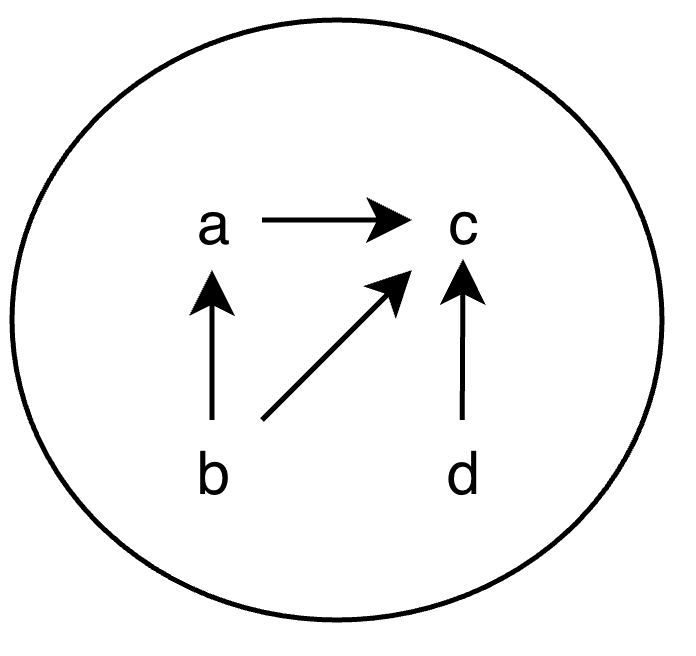
\includegraphics[width=3cm]{images/relazione-transitiva.png}
        \caption{Relazione transitiva}
        \label{fig:relazione-transitiva}
    \end{subfigure}
    \hspace{1.5cm}
    \begin{subfigure}{.3\textwidth}
        \centering
        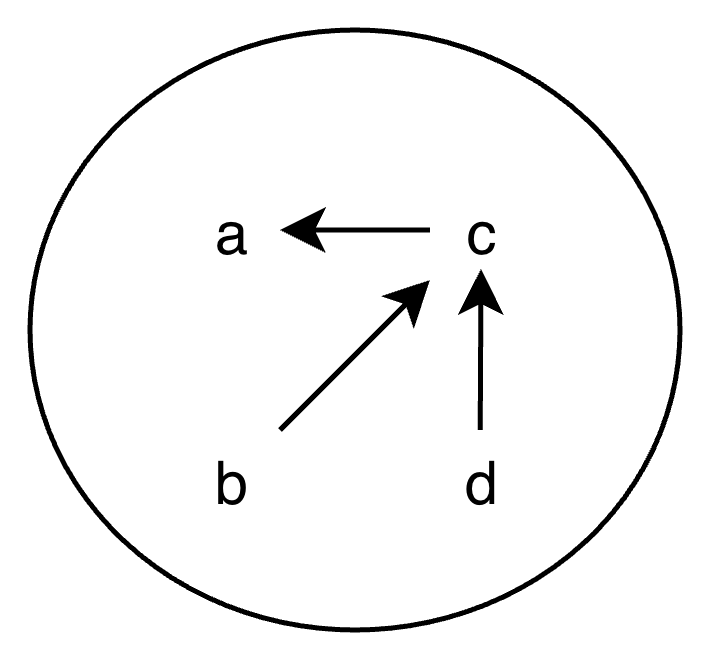
\includegraphics[width=3cm]{images/relazione-non-transitiva.png}
        \caption{Relazione non transitiva}
        \label{fig:relazione-non-transitiva}
    \end{subfigure}
\end{figure}
\newpage
\begin{example}
Alcuni esempi di relazioni transitiva:
    \begin{itemize}
        \item L'Identità di A $Id_A: A \leftrightarrow A$ è transitiva.
        \item La relazione completa $A$ X $A:A \leftrightarrow A$ è transitiva.
        \item La relazione vuota $\O: A \leftrightarrow A$ è transitiva.
        \item La relazione minore $<: \mathbb{N} \leftrightarrow \mathbb{N}$ è transitiva.
        \item La relazione minore-uguale $\leq: \mathbb{N} \leftrightarrow \mathbb{N}$ è transitiva.
        \item La relazioni di amicizia su facebook FbFreind: FB $\leftrightarrow$ FB non è transitiva perché se te sei amico di una persona e questa persona ha amico un altro utente non necessariamente te sei amico di quest'altro utente.
        \item La relazioni di follow su instagram IGFollow: IG $\leftrightarrow$ IG non è transitiva perché se te hai come follow una persona e questa persona ha come follow un altro utente non necessariamente te sei hai come follow di quest'altro utente.
    \end{itemize}
\end{example}

\subsubsection{Anti-simmetrica}
Dato un inseme A, una relazione $R: A \leftrightarrow A$ possiamo definirla come:
\begin{definition}[Anti-simmetrica]
    R è una relazione \textbf{anti-simmetrica} se per tutti gli $a,b \in A$ vale che se $(a, b) \in R$ e $(b, a) \in R$ allora $a = b$
    \begin{center}
        $\forall \: a,b \in A . (a, b) \in R \land (b, a) \in R \Rightarrow a = b$
    \end{center}
\end{definition}
Rappresentiamo \textbf{graficamente} ora una relazione anti-simmetrica. \\Dato un insieme $A$ di partenza dove $A = \{a, b, c, d\}$:
\begin{itemize}
    \item Il caso [\ref{fig:relazione-anti-simmetrica}] è anti-simmetrica perché la premessa è negata, quindi per le varie coppie di valori non esistono coppie simmetriche.
    \item Il caso [\ref{fig:relazione-non-anti-simmetrica}] non è anti-simmetrica perché esiste sia la coppia $(a,b)$ e $(b,a)$ ma a è diverso da $b$.
\end{itemize}
\begin{figure}[h!]
    \vspace{-10pt}
    \centering
    \begin{subfigure}{.3\textwidth}
        \centering
        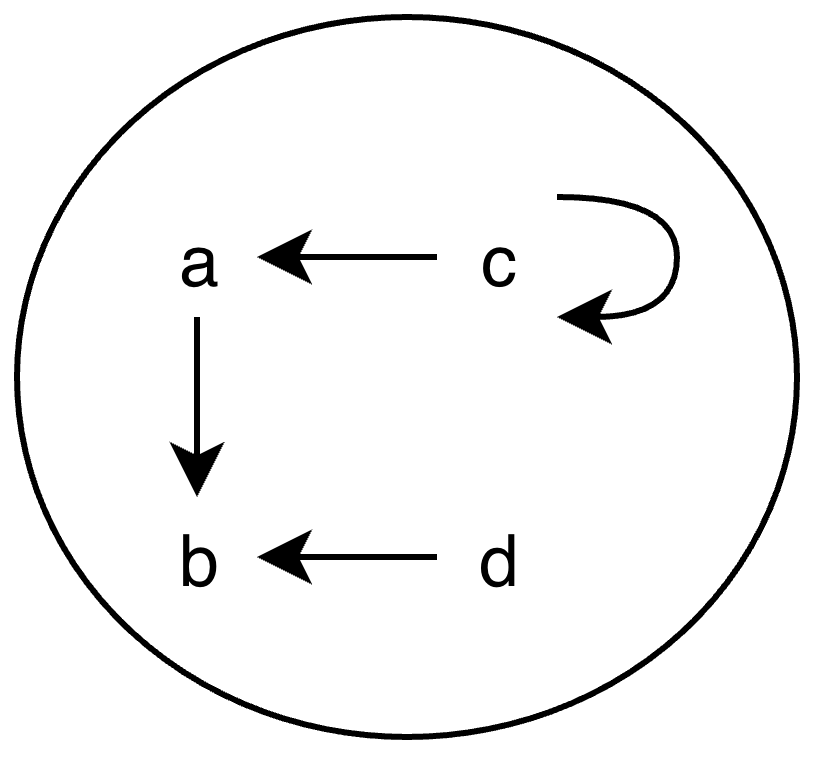
\includegraphics[width=3cm]{images/relazione-anti-simmetrica.png}
        \caption{Relazione anti-simmetrica}
        \label{fig:relazione-anti-simmetrica}
    \end{subfigure}
    \hspace{1.5cm}
    \begin{subfigure}{.3\textwidth}
        \centering
        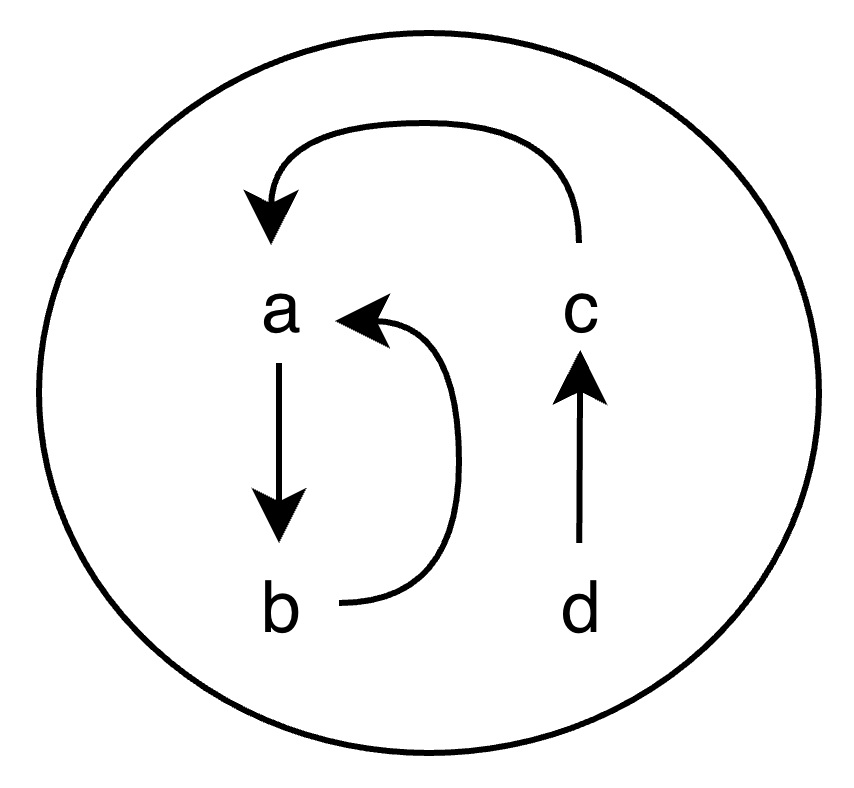
\includegraphics[width=3cm]{images/relazione-non-anti-simmetrica.png}
        \caption{Rel. non anti-simmetrica}
        \label{fig:relazione-non-anti-simmetrica}
    \end{subfigure}
\end{figure}
\begin{example}
Alcuni esempi di relazioni anti-simmetrica:
    \begin{itemize}
        \item L'Identità di $A Id_A: A \leftrightarrow A$ è anti-simmetrica.
        \item La relazione completa $A \times A:A \leftrightarrow A$ non è anti-simmetrica perchè sicuramente esisterà sia $(a,b)$ che $(b,a)$ ma non necessariamente $a = b$.
        \item La relazione vuota $\O: A \leftrightarrow A$ è anti-simmetrica.
        \item La relazione minore $<: \mathbb{N} \leftrightarrow \mathbb{N}$ è anti-simmetrica \footnote{Ricorda che se cade la premessa allora la conclusione è sempre vera per le leggi logiche sugli operatori}.
        \item La relazione minore-uguale $\leq: \mathbb{N} \leftrightarrow \mathbb{N}$ è anti-simmetrica.
    \end{itemize}
\end{example}

\subsection{Teorema di caratterizzazione}
\begin{theorem}[Teorema di caratterizzazione]\label{Teorema-caratterizzazione}
    Pero tutti gli insiemi $A$ e per tutte le relazioni $R: A \rightarrow A$ vale che:
    \begin{enumerate}
        \item $R$ è \textbf{riflessiva} $\Longleftrightarrow Id_A \subseteq R$.
        \item $R$ è \textbf{simmetrica} $\Longleftrightarrow R \subseteq R^{op}$ (o anche $R^{op} \subseteq R, R = R^{op}$).
        \item $R$ è \textbf{transitiva} $\Longleftrightarrow R;R \subseteq R$.
        \item $R$ è \textbf{anti-simmetrica} $\Longleftrightarrow R \cap R^{op} \subseteq Id_A$.
    \end{enumerate}
\end{theorem}
\begin{demostration}[Simmetrica]
Proviamo a dimostrare il punto 2 quindi che R è \textbf{simmetrica} $\Longleftrightarrow$ $R \subseteq R^{op}$ (o anche $R^{op} \subseteq R, R = R^{op}$).\\\\
Per effettuare questa dimostrazione andiamo a dimostrare i due sensi dell'implicazione (in due sensi della freccia $\Longleftrightarrow$).
\begin{itemize}
    \item $\forall \: (a,b) \in R \Longrightarrow (b,a) \in R \Longrightarrow R \subseteq R^{op}$.\\
    Noi sappiamo che per la proprietà simmetrica che per ogni coppia di valori (a,b) dovrà esistere (b,a), quindi l'insieme R sarà composto da una serie di coppie e i loro opposti. Da qui deduciamo come se $(b,a) \in R$ e $(a,b) \in R$ e l'opposto di R, $R^{op}$, conterrà ugualmente tutte le coppie di R soltanto invertite (per la definizione di opposto), farà si che, essendo già presenti le coppie di valori invertite in R, $R \subseteq R^{op}$. In maniera più formale:
    $\forall (a,b) \in R$ sarà presente un $\forall (a,b) \in R^{op}$ e $\forall (b,a) \in R$ sarà presente un $\forall (b,a) \in R^{op}$ per la definizione di op e di simmetria.
    \item $R \subseteq R^{op} \Longrightarrow \forall \: (a,b) \in R \Longrightarrow (b,a) \in R $.\\
    Per dimostrare la proprietà simmetrica partendo da $R \subseteq R^{op}$ consideriamo che: $(a,b) \in R$ per assunzione $(a,b) \in R^{op}$ ma per definizione di opposto, per far in modo che $(a,b) \in R$ allora $(b,a) \in R$, è così dimostrato anche questo senso dell'implicazione.
 \end{itemize}
\end{demostration}

\subsection{Chiusure}
Le chiusure servono per rendere una relazione in un determinato modo tra riflessiva, simmetrica transitiva, applicando delle operazioni fra insiemi.
\subsubsection{Chiusura riflessiva}
La chiusura riflessiva di $R$ è il modo "minimale" per rendere $R$ riflessiva.
\begin{definition}[Chiusura riflessiva]
    Sia $R: A \leftrightarrow A$ una relazione su in insieme $A$, la chiusura \textbf{riflessiva} di $R$ è la relazione $R \cup Id_A$
\end{definition}
\begin{example}
Alcuni esempi di chiusure riflessive:\\
$Id_A: A \leftrightarrow A = Id_A$
\hspace{.7cm}
$A: A \leftrightarrow A = A \times A$
\hspace{.7cm}
$\O: A \leftrightarrow A = Id_A$ \\
$<: \mathbb{N} \leftrightarrow \mathbb{N} = \leq$
\hspace{.7cm}
$\leq: \mathbb{N} \leftrightarrow \mathbb{N}$ = $\leq$
\end{example}
\begin{note}
Nota che per ogni $S: A \longleftrightarrow A$, se $R \subseteq S$ ed $R$ è riflessiva, allora $R \cup Id_A \subseteq S$ 
\end{note}

\subsubsection{Chiusura simmetrica}
La chiusura simmetria di $R$ è un metodo "minimale" per rendere $R$ simmetrica.
Sia $R: A \longleftrightarrow A$ una relazione su in insieme $A$:
\begin{definition}[Chiusura simmetrica]
    Sia $R: A \longleftrightarrow A$ una relazione su in insieme A, la chiusura \textbf{simmetrica} di $R$ è la relazione $R \cup R^{op}$
\end{definition}
\begin{example}
Alcuni esempi di chiusure riflessive:\\
$Id_A: A \longleftrightarrow A$ = $Id_A$
\hspace{.7cm}
$A: A \longleftrightarrow A = A \times A$
\hspace{.7cm}
$\O: A \longleftrightarrow A = \O$ \\
$<: \mathbb{N} \longleftrightarrow \mathbb{N} = \neq$
\hspace{.7cm}
$\leq: \mathbb{N} \longleftrightarrow \mathbb{N} = \mathbb{N} \times \mathbb{N}$
\end{example}

\begin{note}
Nota che per ogni $S: A \longleftrightarrow A$, se $R \subseteq S$ ed $R$ è simmetria, allora $R \cup R^{op} \subseteq S$ 
\end{note}

\subsubsection{Chiusura transitiva}
Per arrivare a capire come opera la chiusura transitiva bisogna partire da un'intuizione. La proprietà transitiva intanto dice in maniera informale che $\forall x,y \in A \times A. \exists (x,y)$ se $x$ "può raggiungere" $y$ in $R$; capiamo dunque come la chiusura transitiva arricchisce $R$ con tutte le coppie $(x,y)$ tali che $y$ è raggiungibile da $x$ seguendo degli archi.\\ \\
Sia data dunque una relazione $R: A \leftrightarrow A$ dove $R = \{(a,b), (b,c), (c,d), (d,e), (d,f)\}$, e rappresentiamo graficamente i vari "passaggi per rendere tale relazione transitiva.
\begin{figure}[h!]
    \centering
    \begin{subfigure}{.3\textwidth}
        \centering
        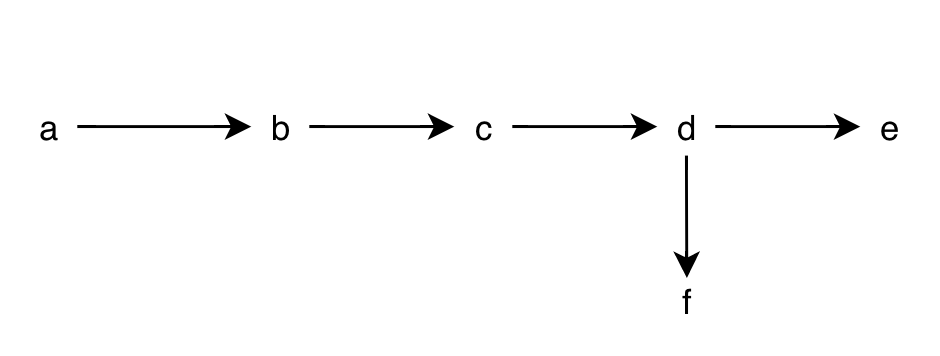
\includegraphics[width=5cm]{images/chiusura-transitiva-1.png}
        \caption{$R$}
    \end{subfigure}
    \hfill
    \begin{subfigure}{.3\textwidth}
        \centering
        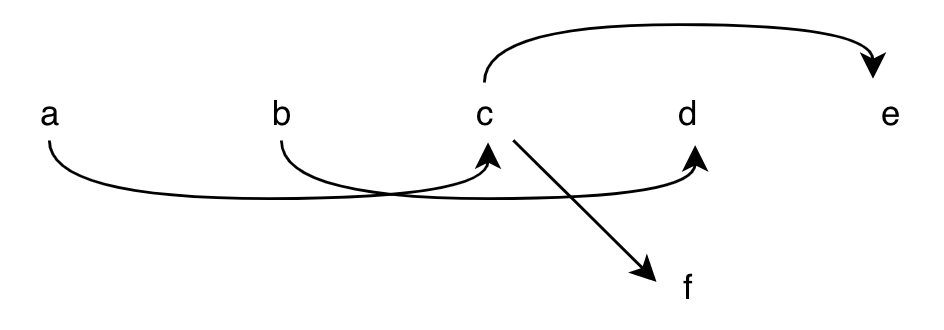
\includegraphics[width=5cm]{images/chiusura-transitiva-2.png}
        \caption{$R;R$}
    \end{subfigure}
    \hfill
    \begin{subfigure}{.3\textwidth}
        \centering
        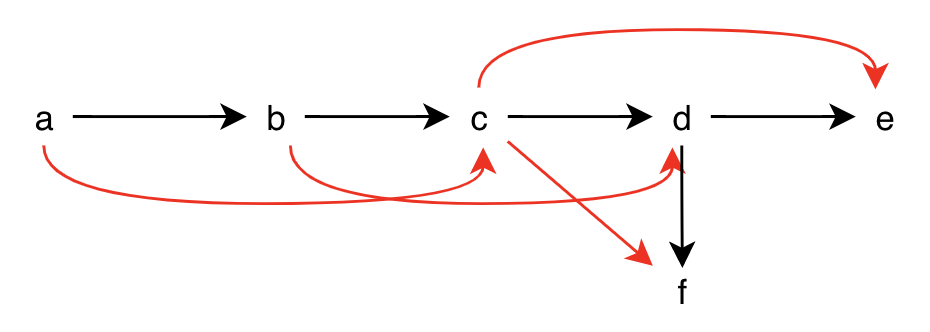
\includegraphics[width=5cm]{images/chiusura-transitiva-3.png}
        \caption{$R \cup R;R$}
    \end{subfigure}
    \hfill
    \begin{subfigure}{.3\textwidth}
        \vspace{15pt}
        \centering
        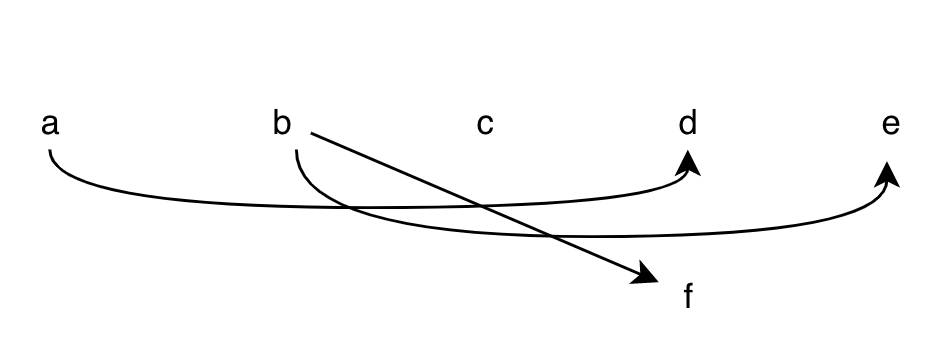
\includegraphics[width=5cm]{images/chiusura-transitiva-4.png}
        \caption{$(R;R);R$}
    \end{subfigure}
    \hfill
    \begin{subfigure}{.3\textwidth}
        \vspace{15pt}
        \centering
        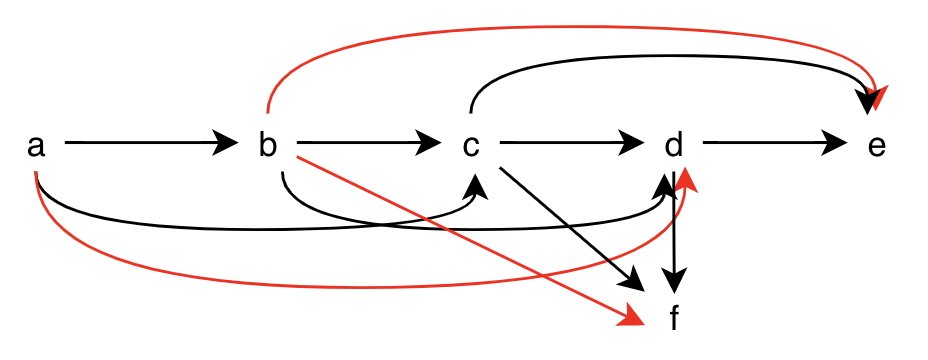
\includegraphics[width=5cm]{images/chiusura-transitiva-5.png}
        \caption{$R \cup R;R \cup R;R;R$}
    \end{subfigure}
    \hfill
    \begin{subfigure}{.3\textwidth}
        \vspace{15pt}
        \centering
        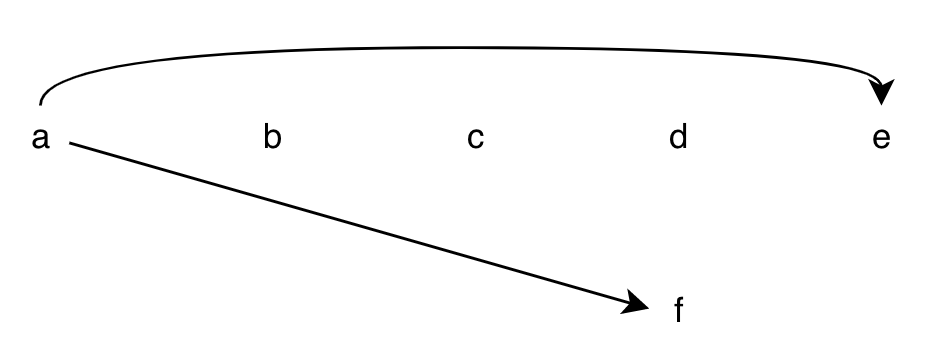
\includegraphics[width=5cm]{images/chiusura-transitiva-6.png}
        \caption{$((R;R);R);R$}
    \end{subfigure}
    \hfill
    \begin{subfigure}{.3\textwidth}
        \vspace{15pt}
        \centering
        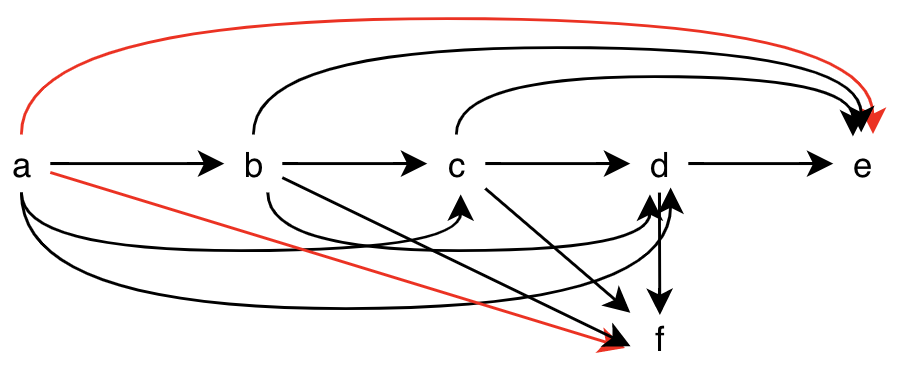
\includegraphics[width=5cm]{images/chiusura-transitiva-7.png}
        \caption{$R \cup R;R \cup R;R;R \cup R;R;R;R$}
    \end{subfigure}
    \hspace{2cm}
    \begin{subfigure}{.3\textwidth}
        \vspace{15pt}
        \centering
        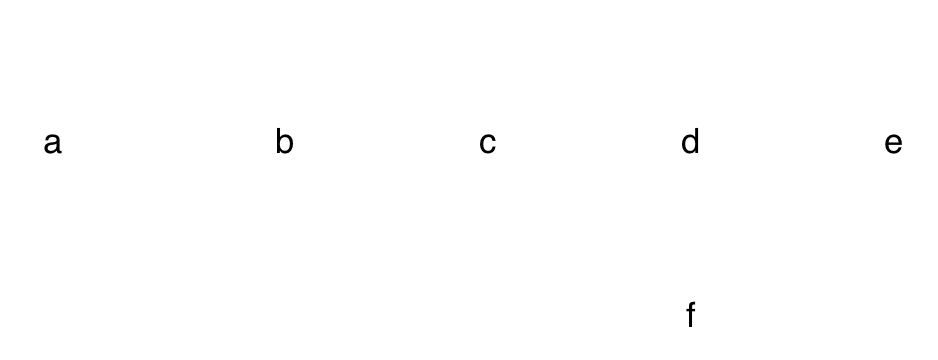
\includegraphics[width=5cm]{images/chiusura-transitiva-8.png}
        \caption{$(((R;R);R);R);R$}
    \end{subfigure}
\end{figure}
\\
Come si vede nelle sequenza di passi sopra, il metodo per fra diventare una relazione transitiva si basa sul ripetere una serie di composizioni ed unirle fra loro finché non si raggiunge uno stato o di vuoto (come in questo caso) o di loop. Questo genere di operazione può essere definita in modo più formale tramite la composizione n-aria di relazione.
\begin{definition}[Composizione n-aria di relazione]
    Sia $A$ un insieme e $R: A \leftrightarrow A$ una relazione su $A$, $\forall n \in \mathbb{N}$, la composizione n-aria $R^n$ è definita induttivamente come:
    \begin{enumerate}
        \item \underline{Caso base:} $R^0 = Id_A$
        \item \underline{Passo induttivo:} $R^{n+1} = R;R^n$
    \end{enumerate}
\end{definition}
\begin{example}
$R^0 = Id_A$ \hspace{.3cm} $R^1 = R;Id_A = R$ \hspace{.3cm} $R^2 = R;R$ \hspace{.3cm} $R^3 = R;R;R$ e così via.
\end{example}
Ora possiamo definire la chiusura transitiva.
\begin{definition}[Chiusura transitiva]
    Sia $R: A \leftrightarrow A$ una relazione su un insieme $A$, la chiusura transitiva di $R$ è la relazione definita come $R^{+} = \bigcup\limits_{n \in \mathbb{N}^+} R^{n}$ con $\O \notin R^{+}$.
\end{definition}
\begin{example}
Alcuni esempi di chiusure transitiva:\\
$Id_A^+ = Id_A$ \hspace{.7cm} $(A \times A)^+:A\leftrightarrow A = A \times A$ \hspace{.7cm} $(\O: A \leftrightarrow A)^+$ = $\O$
\end{example}

\subsection{Stella di Kleene}
\begin{definition}[Stella di Kleene]
    Sia $A$ un insieme ed $R: A \leftrightarrow A$ una relazione su $A$. La chiusura (o stella) di Kleene è la combinazione della chiusura riflessiva e transitiva di R ed è definita come:
    \begin{center}
         $R^\ast = \bigcup\limits_{n \in \mathbb{N}} R^n$ $\longrightarrow$ $R^\ast = (R^+) \cup (Id_A)$
    \end{center}
\end{definition}
\begin{example}
Facciamo un esempio in cui consideriamo l'insieme $A = \{a,b,c,d\}$ ed applichiamo la stella di Kleene alla relazione $R = \{(a,b),(a,d),(b,c)\}$.
\end{example}
\begin{figure}[h!]
    \vspace{-20pt}
    \begin{subfigure}{.3\textwidth}
        \centering
        \includegraphics[width=4cm]{images/stella-Kleene-1.png}
        \caption{$R$ di partenza}
    \end{subfigure}
    \hfill
    \begin{subfigure}{.3\textwidth}
        \centering
        \includegraphics[width=4cm]{images/stella-Kleene-2.png}
        \caption{$R$ di partenza + transitiva (rosso)}
    \end{subfigure}
    \hfill
    \begin{subfigure}{.3\textwidth}
        \centering
        \includegraphics[width=4cm]{images/stella-Kleene-3.png}
        \caption{$R$ di partenza + transitiva (rosso) + riflessiva (verde)}
    \end{subfigure}
\end{figure}

\subsubsection{Applicazione al while}
Prendiamo come esempio questo pezzo di codice while:
\begin{center}
    while ($x \geq 2$) do $\{x = x - 2\}$
\end{center}
Andiamo ora a definire i 3 componenti di questo ciclo.
\begin{itemize}
    \item $C = \{(x, x-2) \mid x \in \mathbb{Z}\}: \mathbb{Z} \leftrightarrow \mathbb{Z}$.
    Identifica il \textbf{corpo} del while, cioè $x = x - 2$, ovvero la parte eseguita ad ogni iterazione.
    
    \item $G = \{(x,x) \mid x \in \mathbb{Z} \land x \geq 2\}: \mathbb{Z} \leftrightarrow \mathbb{Z}$. Identifica la \textbf{guardia}, cioè $x \geq 2$. Si può notare che $G \subseteq Id_{\mathbb{Z}}$, associando coppie di valori uguali, l'unica cosa che contraddistingue $G$ dall'identità è che i valori devono soddisfare la condizione $x \geq 2$.
    
    \item $\overline{G} = \{(x,x) \mid x \in \mathbb{Z} \land x < 2\} : \mathbb{Z} \leftrightarrow \mathbb{Z}$.
    Identifica la \textbf{negazione della guardia} che sarebbe $\overline{G} = Id_{\mathbb{Z}} \setminus G$ cioè tutti i valori che non rispettano la condizione del while.
\end{itemize}
Utilizziamo i 3 componenti appena scritti per andare a definire il pezzo di programma sopra come una relazione.
\begin{equation}\label{while-relazione}
    W = (G;C)^\ast;\overline{G}:\mathbb{Z}\leftrightarrow \mathbb{Z}
\end{equation}
Spieghiamo velocemente la forma scritta sopra [\ref{while-relazione}]. L'obbiettivo è ottenere una relazione che associ un valore consentito dalla guardia al valore finale che uscirà dal while.\\
La prima composizione che troviamo $(G;C)$ è una relazione che dato una qualsiasi numero che rispetti le regole scritte nella guardia restituisce quel numero meno $2$ ($x = x - 2$); andando poi ad applicare la stella di Kleene su quella relazione, $(G;C)^\ast$ stiamo semplicemente aggiungendo la proprietà transitiva e riflessiva all'insieme, quindi per qualsiasi numero che rispetta le condizioni della guardia esisteranno delle coppie per tutti i "cicli" che il while permette, facciamo un esempio: prendiamo $x = 6$, il valore di $x$ rispetta la guardia perché $x \in \mathbb{Z}$ e $x \geq 2$, inoltre, per la prima composizione, esisterà anche la coppia $(x, x-2)$ e cioè $(6,4)$; ora, visto che la relazione è composta da tutti i numeri appartenenti a $\mathbb{Z}$ esisterà anche la coppia con partenza $x = 4$ e quindi formata da $(4,2)$ e così anche le coppie $(2,2)$ e $(2,0)$; se applichiamo quindi la proprietà transitiva si andranno allora a creare le coppie $(6,4), (6,2)$ e $(6,0)$ che possiamo vedere che sono i vari passaggi del while.\\
Arrivati a questo punto però noi vogliamo ottenere una relazione che da un valore restituisca il risultato finale del ciclo. Quindi, riferendosi all'esempio di prima, basterà "eliminare" tutte le coppie "intermedie", e questo si fa con l'ultima composizione, $(G;C)^\ast;\overline{G}$ dove $;\overline{G}$ permette di creare coppie fra i valori di partenza e il valore che non rispetta più la condizione del while, quindi $(6,0), (4,0), \ldots$
\begin{demostration}
    Andiamo ora a dimostrare che per ogni coppia $(a,b) \in \mathbb{Z} \times \mathbb{X}$, $(a,b) \in W$ se e solo se il programma while eseguito a partite da uno stato in cui $x = a$ termina in uno stato in cui $x = b$. \\\\
    
    \textbf{Caso 1°} (\underline{$x < 2$}) - Quello che dobbiamo dimostrare in questo caso è che le coppie $(a,a) \in W$ perché dati dei valori inferiori a 2 il ciclo non parte e quindi restituirà lo stesso valore.\\ \\ In questo caso teoricamente per la legge con cui è costruita la relazione G, $(a,a) \neq G$ e per cioè si verifica anche la condizione $(a,a)\neq G;C$, però nel caso $(G;C)^*$ si aggiunge all'insieme anche tutta $Id_{\mathbb{Z}}$ per la proprietà della stella di Kleene, $Id_{\mathbb{Z}} \subseteq (G;C)^*$, allora arriviamo a vedere che $(a,a) \in (G;C)^*$ e che $(a,a) \in \overline{G}$ (questo perché a sono i valori minori di 2 e quindi rispettano la legge della relazione $\overline{G}$) quindi di conseguenza $(a,a) \in (G;C)^*;\overline{G}$ come desiderato. $\blacksquare$ \\\\
    
    \textbf{Caso 2°} (\underline{$x \geq 2$}) - In questo caso dobbiamo invece dimostrare l'appartenenza all'insieme W di tutte le coppie con un x di partenza valido per l'attivazione del ciclo while.\\\\
    
    Questa seconda casistica si dimostra in maniera intuitiva. Vediamo come prima cosa che $(a,a) \in G$ e $(a,a-2) \in C$ quindi $(a,a-2) \in (G;C)$, quindi per ogni $a \geq 2$ si andranno a costruire i vari passaggi del while, descrivibile come $(G;C)^n$ con $n \in \mathbb{N}^+$ dove $n$ è l'n-esima iterazione. Ad esempio:
    \begin{table}[h!]
        \centering
        \begin{tabular}{c c}
            $(6,4) \: \: \in \: \: (G;C)^1$ & $(7,5) \: \: \in \: \: (G;C)^1$  \\
            $(6,2) \: \: \in \: \: (G;C)^2$ & $(7,3) \: \: \in \: \: (G;C)^2$  \\
            $(6,0) \: \: \in \: \: (G;C)^3$ & $(7,1) \: \: \in \: \: (G;C)^3$ 
        \end{tabular}
    \end{table}
    \begin{note}
    \vspace{-10pt}
    Nota che nell'esempio sopra $(6, -2) \notin (G;C)^4$ in quanto $(0, -2) \notin G;C$
    \end{note}
    Ora per concludere la dimostrazione basta considerare che la composizione $(G;C)^\ast;\overline{G}$ va ad associare ogni interazione valida all'interno di while $(a,a-2)$ con i valori che non la validano (che si trovano nella relazione $\overline{G}$) quindi seguendo l'esempio sopra $(7,1) \in W$ e $(6,0) \in W$. Poiché questo ragionamento può essere applicato ag ogni numero pari o dispari maggiore o uguale a $2$, questo conclude anche questo caso della dimostrazione. $\blacksquare$
\end{demostration}

\subsubsection{Leggi stella di Kleene}
Per tutti gli insiemi A e le relazioni $R: A \longleftrightarrow A$ e $S: A \longleftrightarrow A$ valgono le seguenti uguaglianze.
\begin{table}[h!]
    \centering
    \setlength{\tabcolsep}{10pt}
    \renewcommand{\arraystretch}{1.3}
    \begin{tabular}{|c|c|}
        \hline
        \textbf{Riflessività} & $Id_A \subseteq R^*$ \\
        \textbf{Transitività} & $R^*;R^* \subseteq R^*$ \\
        \textbf{Chiusura} & $R \subseteq R^*$ \\
        \textbf{Indempotenza} & $(R^*)^* = R^*$ \\
        \textbf{*-id} & $Id_A^* = Id_A$ \\
        \textbf{*-compl} & $(A$ X $A)^*$ = $A$ X $A$  \\
        \textbf{*-vuoto} & $\O_{A;A}^* = Id_A$ \\
        \textbf{Distributività di * su $\cup$} & $R^* \cup S^* \subseteq (R \cup S)^*$ \\
        \textbf{Distributività di * su $\cap$} & $(R \cap S)^* \subseteq R^* \cap S^*$ \\
        \textbf{Distributività di * su $.^{op}$} & $(R^*)^{op} = (R^{op})^*$ \\
        \hline
    \end{tabular}
    \caption{Leggi stella di Kleene}
    \label{tab:leggi-stella-Kleene}
\end{table}

\subsection{Relazioni di equivalenza}
\begin{definition}[Relazioni di equivalenza]
    Sia A un insieme $R: A \leftrightarrow A$ una relazione su $A$, si dice che $R$ è una relazione di equivalenza se \textbf{riflessiva}, \textbf{simmetrica}, \textbf{transitiva}. 
\end{definition}
\begin{example}
Alcuni esempi di relazioni di equivalenza:\\
$Id_A: A \leftrightarrow A$ SI \hspace{.7cm} $A: A \leftrightarrow A$ SI \hspace{.7cm} $\O: A \leftrightarrow A$ NO (SI se $A=\O$) \\
$<: \mathbb{N} \leftrightarrow \mathbb{N}$ NO perché non riflessiva \hspace{.7cm} $\leq: \mathbb{N} \leftrightarrow \mathbb{N}$ NO perché non simmetrica
\end{example}
\begin{example}
	$A = \{a, b, c, d\}$ $R=\{(a,a), (b,b), (a,b), (b,a), (c,c), (d,d)\}$ è una relazione di equivalenza.
\end{example}

\subsubsection{Classe di equivalenza}
\begin{definition}[Classe di equivalenza]
    Data $R: A \leftrightarrow A$ una relazione di equivalenza, ed $a \in A$, la classe di equivalenza di $a$ si definisce come l'insieme: 
    \begin{equation}
        [a]_R = \{b \in A \mid (a,b) \in R\}
    \end{equation}
\end{definition}
\begin{example}
    Prendiamo $A = \{a,b,c,d\}$ ed $R = \{(a,b), (b,a), (a,a), (b,b), (c,c), (d,d)\}$\\
    Le classi di equivalenza saranno per ogni elemento di A le seguenti:\\
    $[a]_R = \{a,b\}$ \hspace{.5cm} $[b]_R = \{a,b\}$ \hspace{.5cm} $[c]_R = \{c\}$ \hspace{.5cm} $[d]_R = \{d\}$
\end{example}
\begin{example}
    Altri esempi di classi di equivalenza. Dato un insieme A si considerino le relazioni $Id_A$ e la relazione $A$ X $A$, per tutti gli $a \in A$ vale che: \: \: \:
    $[a]_{Id_A} \: = \: \{a\}$ \hspace{.7cm} $[a]_{A \times A} \: = \: A$
\end{example}

\subsubsection{Teorema di biiezione}
Conoscendo la definizione di partizione e di classe di equivalenza possiamo osservare che:
\begin{itemize}
    \item L'insieme di tutte le classi di equivalenza di $R$ definisce una partizione dell'insieme $A$.
    \[EC_R = \{[a]_r \:|\: a \in A\}\]
    \item Viceversa, ogni partizione di $A$ definisce una relazione di equivalenza.
    \begin{center}
        $Rf = \{(a,b) \in A \times A \mid \exists i a,b \in A_i\}$
    \end{center}
\end{itemize}

\begin{theorem}[Teorema di biiezione]
    Sia A un insieme, ERel(A) l'insieme di tutte le relazioni di equivalenza su A, Part(A) l'insieme di tutte le partizioni su A. Allora:
    \begin{equation}
        ERel(A) \cong Part(A)
    \end{equation}
\end{theorem}

\subsection{Relazioni di ordinamento}
\subsubsection{Ordinamento parziale}
\begin{definition}[Ordinamento parziale]
    Sia $A$ un insieme e $R: A \leftrightarrow A$ una relazione su $A$. Si dice che $R$ è una relazione di ordinamento parziale se è \textbf{riflessiva}, \textbf{transitiva} e \textbf{anti-simmetrica}.
\end{definition}
\begin{note}
    Nota che gli ordinamenti si scrivono utilizzando o il simbolo $\prec$, $\preceq$ oppure $\sqsubset$, $\sqsubseteq$.
\end{note}
\begin{example}
Alcuni esempi di ordinamento parziale:\\
$Id_A: A \leftrightarrow A$ SI \hspace{.7cm} $A \times A: A \leftrightarrow A$ NO  \hspace{.7cm} $\O: A \leftrightarrow A$ NO (SI se $A = \O $) \\
$<: \mathbb{N} \leftrightarrow \mathbb{N}$ NO perché non riflessiva \hspace{.7cm} $\leq: \mathbb{N} \leftrightarrow \mathbb{N}$ SI.
\end{example}
\begin{example}
	Dato un insieme $A = \{a,b,c\} $:
	\begin{itemize}
		\item $R=\{(a,b), (b,c)\}$ NON è una relazione di ordinamento parziale
		\item $S = \{(a,a),(b,b)(a,b),(a,c),(b,c),(c,c)\}$
	\end{itemize} 
\end{example}

\begin{proposition}
Per ogni insieme A, l'inclusione $\mathcal{P}(X)$ è una relazione di ordinamento parziale, e si scrive come:
\begin{center}
    $\{(X,Y) \in \mathcal{P}(X) \times \mathcal{P}(X) \: | \: X \subseteq Y\}$
\end{center}
\end{proposition}
Per capire se la proposizione scritta sopra è vera dobbiamo verificare che la relazione create abbia le proprietà riflessiva, transitiva ed anti-simmetrica.\\ \\
Innanzitutto capiamo cosa crea questo insieme. Essendo il prodotto cartesiano fra due insiemi della parti su un insieme A sarà formato da coppie ordinate costituiate da insiemi (essendo che l'insieme $\mathcal{P}(X)$ è un insieme di insiemi che contiene tutti i possibili insiemi creabili con A), non è però un prodotto cartesiano "completo" ma verranno prese solo le coppie di valori che rispettano la legge $X \subseteq Y$ che vuol dire che in una coppia ordinata (A,B) dove A e B sono due insiemi $A \subseteq B$.Ora che abbiamo capito da cos'è costituita questa relazioni verifichiamo le varie proprietà.
\begin{enumerate}
    \item \textbf{Riflessiva}: la relazione sarà riflessiva perché al suo interno esisteranno tutte le coppie $(A,A)$, $(B,B)$, $(C,C)$ visto che un insieme è sempre sotto insieme uguale a se stesso.
    \item \textbf{Transitiva}: la relazione sarà anche transitiva visto che se prendiamo due coppie ordinate $(A,B)$ e $(B,C)$ dove per le regole della relazione $A \subseteq B$ e $B \subseteq C$ esisterà anche $(A,C)$ visto che se $A \subseteq B \subseteq C$ allora $A \subseteq C$.
    \item \textbf{Anti-simmetrica}: in fine la relazione sarà anche anti-simmetrica perché se esistono coppie $(A,B)$ dove $A \leq B$ non potrà mai esiste una coppia $(B,A)$ perché se $A \subseteq B$ e $A \leq B$, l'insieme B avrà obbligatoriamente elementi in più di A (non in meno perché in quel caso A non sarebbe sotto insieme) quindi, per le regole della relazione, non potrà esistere la coppia $(B,A)$ quindi la premessa è falsa e quindi la conseguenza, per le regole dell'implicazione, è vera. Mentre nel caso in cui $A = B$ la condizione di anti-simmetria è valida per sua stessa definizione.
\end{enumerate}

\subsubsection{Ordinamento}
\begin{definition}[Ordinamento]
    Sia $R: A \leftrightarrow A$ una relazione di ordinamento parziale su un insieme $A$, si dice che $R$ è ordinamento se soddisfa le seguenti proprietà (totalità). Per tutti gli $(a,b) \in A \times A$ vale che $(b,a) \in R$ oppure $(b,a) \in R$. Formalmente:
    \begin{equation}
        \forall (a,b) \in A \times A \times (a,b) \in R \lor (b,a) \in R
    \end{equation}
\end{definition}
\begin{example}
Alcuni esempi di ordinamento:\\
$Id_A: A \longleftrightarrow A$ NO \hspace{.5cm} $A \times A: A \longleftrightarrow A$ Non è un ordinamento parziale  \hspace{.5cm} $\leq: \mathbb{N} \longleftrightarrow \mathbb{N}$ SI \\
$<: \mathbb{N} \longleftrightarrow \mathbb{N}$ Non è un ord. parziale \hspace{.7cm} $\O: A \longleftrightarrow A$ Non è un ord. parziale.
\end{example}

\subsubsection{Ordinamento lessiografico}
\begin{definition}[Ordinamento lessiografico]
    Dato un ordinamento $\sqsubseteq_A: A \longleftrightarrow A$, \textbf{l'ordinamento lessiografico} è: $a_0a_1... a_n \sqsubseteq_{A^*} b_0b_1...b_m$ se esiste $i \in \mathbb{N}$ tale che:
    \begin{enumerate}
        \item $a_j = b_j$ per tutti i $j < i$
        \item $a_i \sqsubseteq_A b_j$ e $a_i \neq b_j$ oppure $i = n+1$ e $n < m$
    \end{enumerate}
\end{definition}
Questo tipo di ordinamento è usato per le parole nei dizionari o negli elenchi. Si usa se dato un insieme A e un ordinamento $\sqsubseteq_A: A \longleftrightarrow A$(ordinamento sui caratteri), si vuole definire un ordinamento $\sqsubseteq_{A^*}: A^* \longleftrightarrow A^*$(ordinamento sulle stringhe) sull'insieme delle stringhe su A.
Noi conosciamo l'ordinamento dei caratteri (l'afabeto), dato questo possiamo, tramite l'ordinamento lessiografico, ordinare le stringhe.
\begin{example}
Dato un $A = \{a,b,c,...,z\}$ con $a \sqsubseteq_A b \sqsubseteq_A c \sqsubseteq_A ... \sqsubseteq_A z$.\\
Allora tramite l'ordinamento lessiografico $alessandro \sqsubseteq_A anna \sqsubseteq_A annarella \sqsubseteq_A ...$
\end{example}